\begin{minipage}{\columnwidth}
\begin{algorithm}[H]
\caption{Accumulate Heuristic Scheduling for Multi-Shuffles}
\label{mhminheap}
	\begin{algorithmic}[1]
	\small
	\Procedure{\Large m\_schedule}{$m, host\_id, p\_reduces, shuffles$}
		\State $m\gets$ partition number of map tasks
		\Comment $shuffles$ is the previous schedule result 
		\ForAll{$r$ in $p\_reduces$}
			\State $r.size \mathrel{+}= shuffles\left[r.rid\right].size$
			\State $new\_prob\gets shuffles\left[r.rid\right].size / r.size$
			\If{$new\_prob\geq r.prob$}
				\State $r.prob\gets new\_prob$
				\State $r.host\_id\gets shuffles\left[r.rid\right].assigned\_host$
			\EndIf
		\EndFor
		\State $M\gets$ $SCHEDULE\left(m, host\_id, p\_reduces\right)$
		\ForAll{$host\_id$ in $M$}
			\Comment Re-shuffle
			\ForAll{$r$ in $M\left[host\_id\right].reduces$}
				\If{$host\neq shuffles\left[r.rid\right].assigned\_host$}
				\State Re-shuffle data to $host$
				\State $shuffles\left[r.rid\right].assigned\_host\gets host$
				\EndIf
			\EndFor
		\EndFor
		\Return $M$
	\EndProcedure
	\end{algorithmic}
\end{algorithm}
\end{minipage}

\section{Implementation}\label{impl}
This section presents an overview of the implementation of SCache -- an open source cross-framework shuffle data management system with a DAG co-scheduler. Here we use Spark as an example of DAG framework to illustrate the work flow of shuffle optimization. We will first present the system overview in Subsection \ref{arch} while the following two subsections focus on the two constraints on memory management.

\begin{figure}
	\centering
	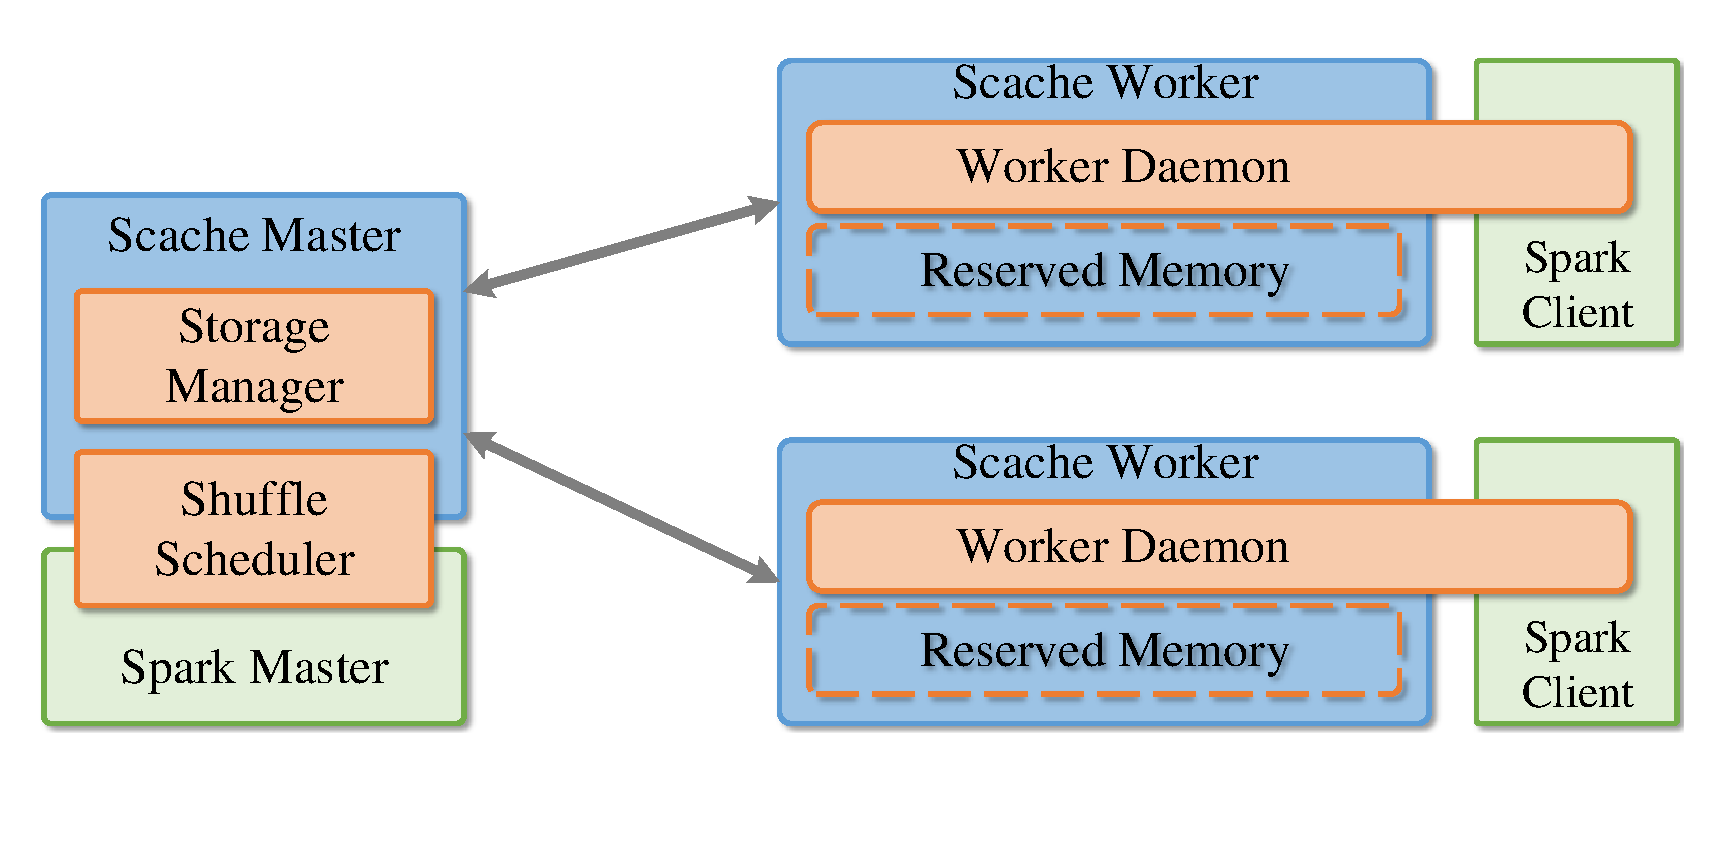
\includegraphics[width=0.8\linewidth]{fig/arch}
	\caption{SCache Architecture}
	\label{fig:arch}
	\vspace{-1em}
\end{figure}

\subsection{System Overview}\label{arch}
SCache consists of three components: a distributed shuffle data management system, a DAG co-scheduler, and a daemon inside Spark. As shown in Figure \ref{fig:arch}, SCache employs the legacy master-slaves architecture like GFS \cite{gfs} for shuffle data management system. 

The master node of SCache coordinates the shuffle blocks globally with application context. The worker node reserves memory to store blocks.
The coordination provides two guarantees: (a)data is stored in memory before tasks start and (b)data is scheduled on-off memory with all-or-nothing and context-aware constraints. 
The daemon bridges the communication between Spark and SCache. The co-scheduler is dedicated to pre-schedule reduce tasks with DAG information and enforce the scheduling results to Spark scheduler.

When a Spark job starts, the DAG will be first generated. 
During the DAG generation, the shuffle dependencies among Resilient Distributed Datasets (RDDs) will be submitted through the daemon process in Spark driver. The SCache master recognizes all shuffle dependencies in a RPC call as a shuffle scheduling unit.
For each shuffle dependency, the shuffle ID, the type of partitioner, the number of map tasks, and the number of reduce tasks are included.  If there is a specialized partitioner, such as RangePartitioner, in the shuffle dependencies, the daemon will insert a sampling application before the dependent RDDs. We will elaborate the sampling procedure in the Section \ref{sampling}.
\hlyellow{
For the hash partitioner, when a map task finishes computing, the shuffle write implementation of Spark is modified to call the SCache API and move data out of Spark executor's JVM through memory copy
}
After that the slot will be released without blocking on disk operations.
When the shuffle map output is received, the SCache worker will notify the master of the block ID and reduce size distribution of this block (see map output in Figure \ref{fig:shuffle}).
If the collected map output data reach the observation threshold, the DAG co-scheduler will run the scheduling Algorithm \ref{hminheap} and \ref{mhminheap} to pre-schedule the reduce tasks and then broadcast the scheduling result to start pre-fetching on each worker.
After that, when a map task is finished, each node will receive a broadcast message. 
SCache worker will filter the reduce tasks ID that will be launched on itself and start pre-fetching shuffle data from the remote. 
To enforce SCache pre-scheduled tasks -- node mapping, we insert some lines of codes in Spark DAG Scheduler.
For RDDs with shuffle dependencies, Spark DAG scheduler will consult SCache master to get the preferred location for each reduce task.

\begin{figure}
	\centering
	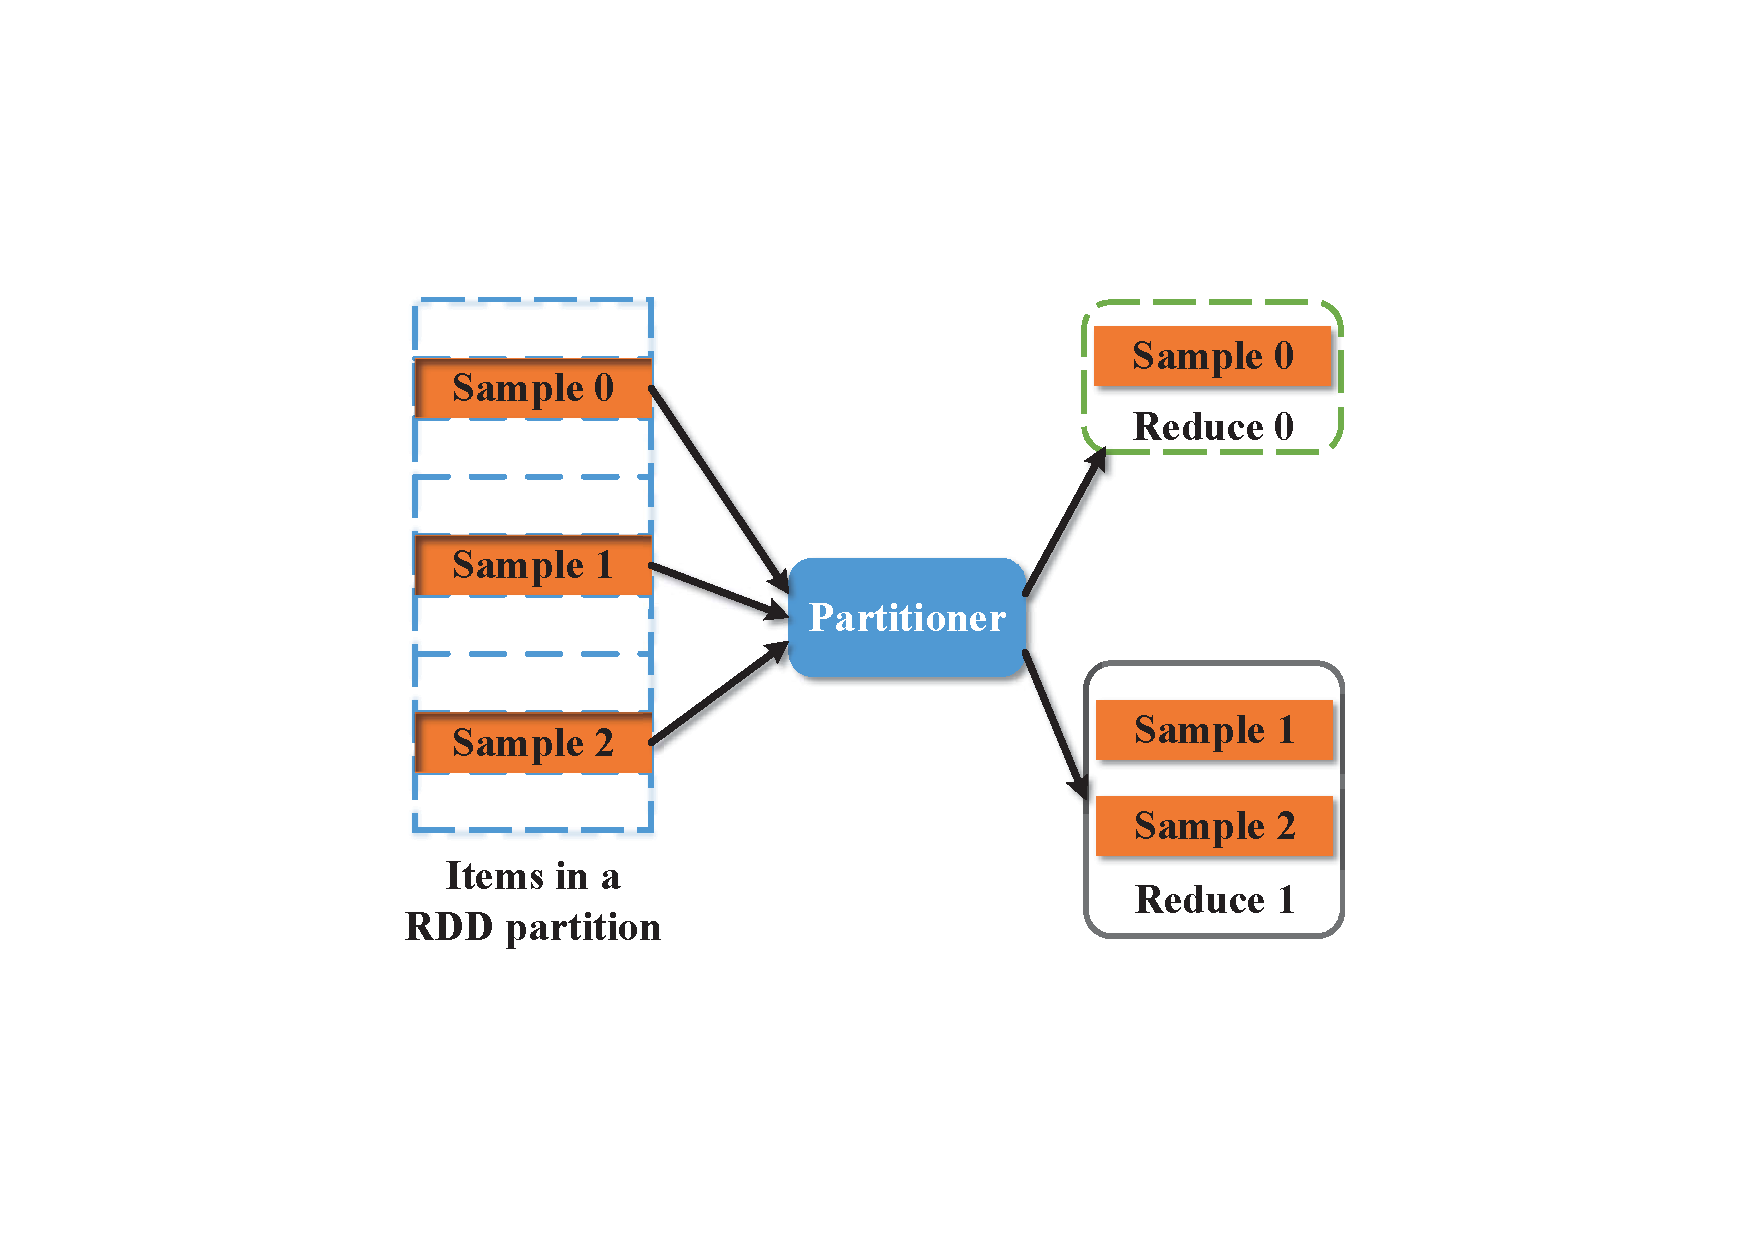
\includegraphics[width=0.6\linewidth]{fig/sample}
	\caption{Reservoir Sampling of One Partition}
	\label{fig:sample}
	\vspace{-1em}
\end{figure}

\subsubsection{Reservoir Sampling}\label{sampling}
If the submitted shuffle dependencies contain a range partitioner or a customized non-hash partitioner, the SCache master will send a sampling request to the daemon in Spark driver. The daemon then inserts a sampling job before the corresponding RDD. The sampling job uses a reservoir sampling algorithm \cite{reservoir} on each partition of RDD. For the sample number, we set the size to $3 \times number\ of\ partitions$ for balancing overhead and accuracy (it can be tuned by configuration). The sampling job randomly selects some items and performs a local shuffle with partitioner (see Figure \ref{fig:sample}). At the same time, the items number is counted as the weight. These sampling data will be aggregated by reduce ID on SCache master to predict the reduce partition size. After the prediction, SCache master will call Algorithm \ref{mhminheap} and \ref{hminheap} to do the scheduling.

% In the case of extreme skew scenario, such as Figure \ref{fig:range_pre_sample}, Heuristic MinHeap trades about 0.05\% percent of stage completion time for 99\% reduction of shuffle data transmission through network by heuristicly swapping tasks.
\subsection{Memory Management}\label{memorymanage}
As mentioned in Section \ref{observation}, though the shuffle size is relatively small, memory management should still be cautious enough to limit the effect of performance of DAG framework.
When the size of cached blocks reaches the limitation of reserved memory, SCache flushes some of them to the disk temporarily, and re-fetches them when some cached shuffle blocks are consumed or pre-fetched. To achieve the maximum overall improvement, SCache leverages two constraints to manage the in-memory data --- all-or-nothing and context-aware-priority.
\subsubsection{All-or-Nothing Constraint}
Memory cached shuffle blocks can speed up the reduce task execution process. But this acceleration of a single task is necessary but insufficient for a shorter stage completion time. Based on the observation in Section \ref{multi}, in most cases one single stage contains multi-rounds of tasks. If one task misses a memory cache and exceeds the original bottleneck of this round, that task might become the new bottleneck and further slow down the whole stage. PACMan \cite{pacman} has also proved that for multi-round stage/job, the completion time improves in steps when $n\times number\ of\ tasks\ in\ one\ round$ of tasks have data cached simultaneously. Therefore, the cached shuffle blocks need to match the demand of all tasks in one running round at least. We refer to this as the all-or-nothing constraint.

According to all-or-nothing constraint, SCache master leverages the pre-scheduled results to determine the bound of each round, and sets corresponding blocks as the minimum unit of storage management.
For those incomplete units, SCache will mark them as the lowest priority.
% Following the all-or-noting constraint can maximum the improvement in stage completion time by using reserved memory efficiently.

\subsubsection{Context-Aware-Priority Constraint}
Unlike the traditional cache replacement schemes such as MIN \cite{min}, the cached shuffle data will only be used once (without failure) in DAG computing. That is, the effort of improving hit rate in most legacy schemes can not benefit DAG application, while their approaches can easily violate the all-or-nothing constraint.
SCache also leverages application context to select victim storage units when the reserved memory is full.

At first, SCache master searches for the incomplete units and flushes all belonging blocks to disk cluster-widely.

If all the units are completed, SCache selects victims based on two factors --- \textit{inter-shuffle units} and \textit{intra-shuffle unit}.
\begin{itemize}[noitemsep]
	\item Inter-shuffle units: SCache master follows the scheduling scheme of Spark to determine the inter-shuffle priority. For a FAIR scheduler, Spark balances the resource among task sets, which leads to a higher priority for those having more tasks unfinished. So SCache sets priorities from high to low in a descending order of remaining storage units of a shuffle unit. For a FIFO scheduler, Spark schedules the task set that is submitted first. So SCache sets the priorities according to the submit time of each shuffle unit.
	\item Intra-shuffle unit: SCache also needs to decide the priority among storage units inside a shuffle unit. According to the task scheduling inside a task set of Spark, the tasks with smaller ID will be scheduled firstly. Based on this, SCache can assign the lower priority to storage units with larger task ID.
\end{itemize}

\subsection{Cost of adapting SCache}
SCache provides API through RPC, such as \textit{putBlock(blockId)}, \textit{getBlock(blockId)}, and \textit{getScheduleResult(shuffleId)}. 
The concise design makes it easy to adapt DAG frameworks to enable SCache optimization. 
For example, it only takes about 500 lines of code in Spark to integrate SCache. 

\ifrevision
\marginnote{60B,C,D,E,F}
\fi

By a glance of Hadoop source code, we believe that the costs of adapting SCache on MapReduce \cite{hadoop} is also acceptable. 
\hlyellow{
The shuffle write and read of MapReduce can be replaced by implementing the interface named} \textit{MapOutputCollector.java} (shuffle write) and \textit{ShuffleConsumerPlugin.java} (shuffle read) using SCache's APIs.
The DAG information can be fetched in \textit{JobImp.java}. The sampling tasks insertion can also be implemented inside the \textit{JobImp.java}. 
As for the co-scheduling, the pre-scheduled results from SCache can be enforced by modifying the \textit{RMContainerAllocator.java}. 

\hlyellow{
Based on the effort of modifying Spark and the feasibility study of Hadoop MapReduce, we believe the cost of adapting SCache is low.
}

\subsection{Discussion of Fault Tolerance}

\ifrevision
\marginnote{60C}
\fi

Since fault tolerance is not a crucial goal of SCache, we have not implemented fault tolerance mechanism. 
We plan to implement SCache master with Apache ZooKeeper \cite{zookeeper} to provide constantly service. 
As for the worker node, a possible way is to select some backup nodes to store replications. 
But the replications can introduce a significant network overhead \cite{availability}.  

\hlyellow{
A more promising way of fault tolerance is to collaborate with the recovery scheme of DAG frameworks. 
If a failure happened inside the SCache worker, SCache daemon cloud blocking the shuffle write/read operations until the worker process restarted.
If a failure happened in the DAG framework, SCache could ignore it and provide shuffle optimization during the recovery job of DAG framework.
Both of the above methods do not violate the correctness of DAG jobs.
}
% For SCache worker, a promising way to prevent failure is to select some backup nodes to store replications of shuffle data during pre-scheduling. In addition, there are also advanced fast recovery techniques such as FineFRC \cite{finefrc}. We leave this to the future work.


% \subsubsection{Fault Tolerance}
% To prevent the machine failure in cluster leading to inconsistency SCache, the master node will log the meta data of shuffle register and scheduling on the disk. Since we remove the shuffle transfer from the critical path of DAG computing, the disk log will not introduce extra overhead to the DAG framworks. Note that the master can be implemented with Apache ZooKeeper \cite{zookeeper} to provide constantly service to DAG framework.
% At the same time, every work node will send a heartbeat to master to report status. If a failure of work node is detected, the master will the do a simple re-schedule. For those scheduled shuffle units, the master assgins the tasks to other workers with more lightweight workload evenly. Then the new assigned worker will fetch the data again. For the incomplete in memory map blocks on the failure node, SCache simply ignore them since DAG framework will schedule the failure map tasks on another node.
